

 The three circles below are congruent and have radius 3:
 \begin{center}
 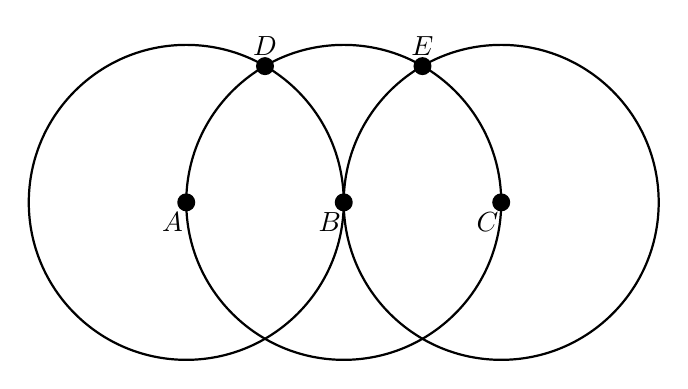
\begin{tikzpicture}
 
 \draw (0,0)[thick] circle (2);
 \draw (2,0)[thick] circle (2);
 \draw (4,0)[thick] circle (2);
      \draw (0,0)[fill=black, thick] circle (1mm) node[below]{$A$\,\,\,\,\,\,}; 
     \draw (2,0)[fill=black, thick] circle (1mm) node[below]{$B$\,\,\,\,\,\,};
         \draw (4,0)[fill=black, thick] circle (1mm) node[below]{$C$\,\,\,\,\,\,};
     \draw (1,1.73)[fill=black, thick] circle (1mm) node[above]{$D$};
     \draw (3,1.73)[fill=black, thick] circle (1mm) node[above]{$E$};
    
\end{tikzpicture}
\end{center}


If $A,B$ and $C$ are the centers of the three circles, then what is the perimeter of the trapezoid $ABCED$ (not drawn)?



\ifsat
	\begin{enumerate}[label=\Alph*)]
		\item  $9\sqrt{3}$
		\item  $12$ 
		\item  $15$%
		\item  Cannot be determined
	\end{enumerate}
\else
\fi

\ifacteven
	\begin{enumerate}[label=\textbf{\Alph*.},itemsep=\fill,align=left]
		\setcounter{enumii}{5}
		\item   $9\sqrt{2}$ 
		\item  $9\sqrt{3}$
		\item  $12$ 
		\addtocounter{enumii}{1}
		\item  $15$%
		\item  Cannot be determined
	\end{enumerate}
\else
\fi

\ifactodd
	\begin{enumerate}[label=\textbf{\Alph*.},itemsep=\fill,align=left]
		\item   $9\sqrt{2}$ 
		\item  $9\sqrt{3}$
		\item  $12$ 
		\item  $15$%
		\item  Cannot be determined
	\end{enumerate}
\else
\fi

\ifgridin
  $15$%
		
\else
\fi

